\section{Phát biểu bài toán}

    \subsection{Mục tiêu và phạm vi}
    Dự án nghiên cứu khả năng sử dụng ảnh camera tại khu vực Ngã Tư Hàng Xanh để theo dõi mức hiện diện của phương tiện và ước lượng thời gian đến một trạng thái đông xe. Hệ thống chuyển ảnh thành số đếm theo loại phương tiện, xây dựng chuỗi thời gian, dự báo diễn biến trong một giờ tiếp theo và trình bày kết quả trên ứng dụng desktop.

    Phiên bản đã triển khai giải quyết một bài toán cụ thể: dự báo chỉ số WTI(Weighted Traffic Index - Chỉ số tải trọng giao thông) trung bình từng phút trong 60 phút tiếp theo, sau đó xác định thời điểm bắt đầu cửa sổ vượt ngưỡng WTI thử nghiệm. Đây là hệ thống nguyên mẫu phục vụ nghiên cứu. Tập dữ liệu chưa có nhãn ùn tắc độc lập, tốc độ dòng xe hoặc thời gian hành trình để xác nhận trạng thái ùn tắc ngoài thực tế.

    \begin{figure}[htbp]
        \centering
        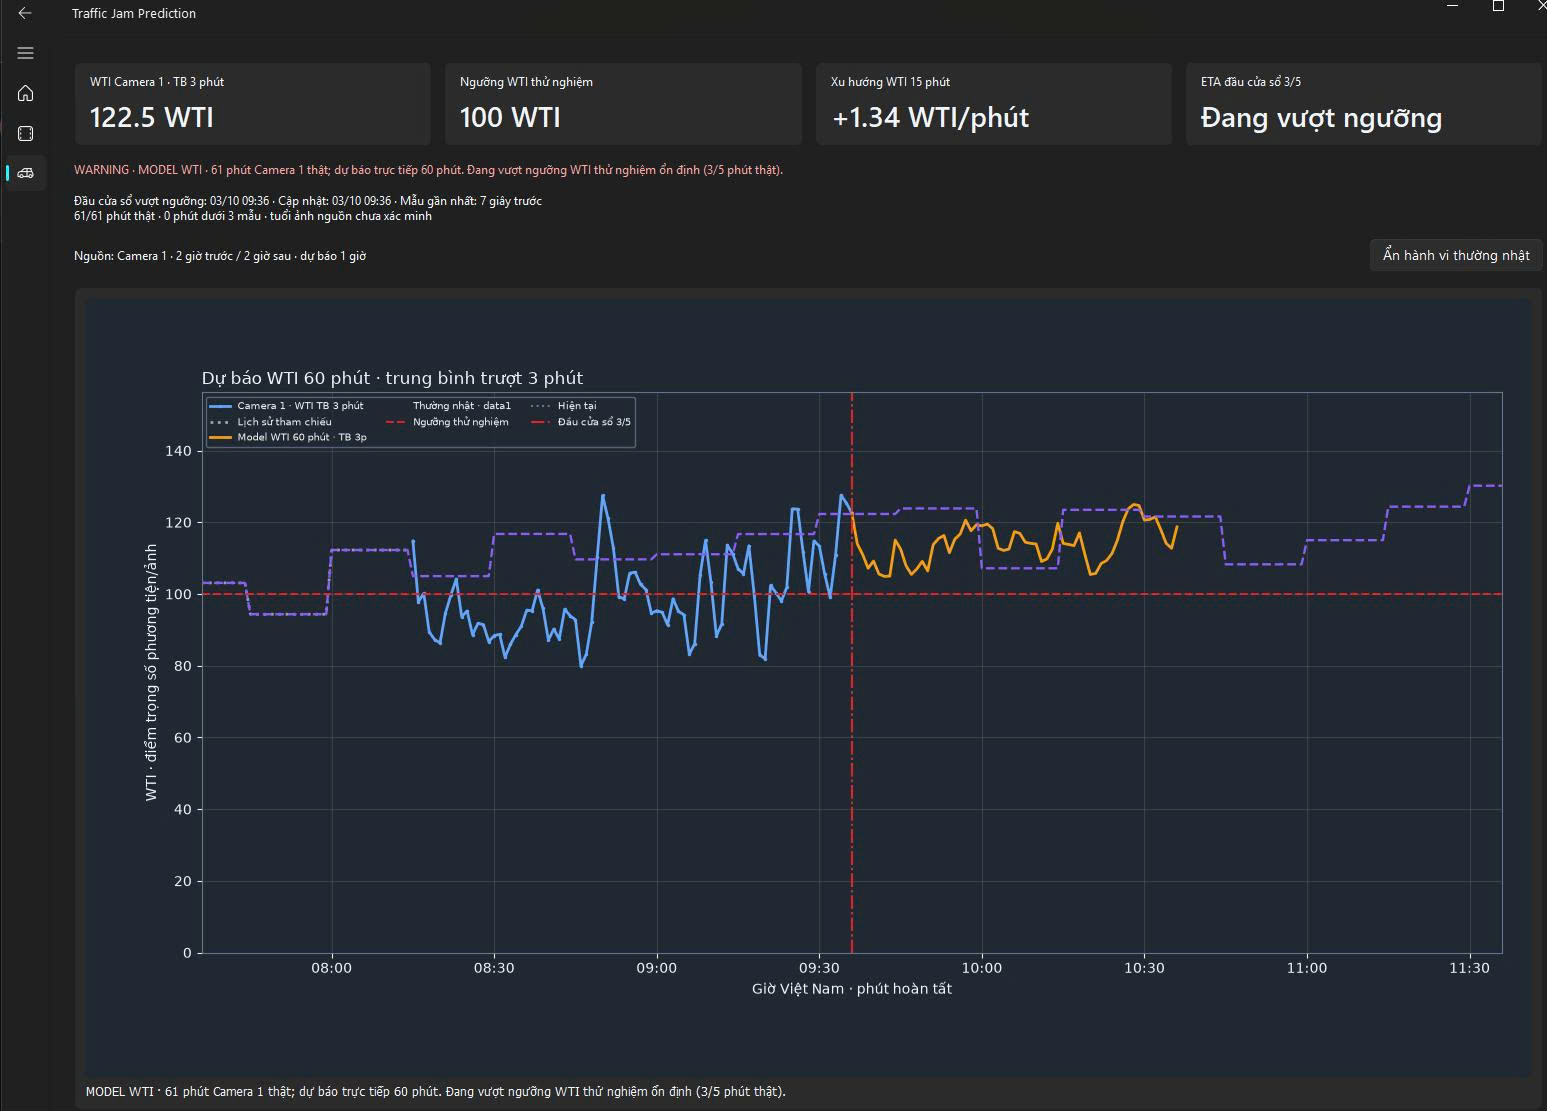
\includegraphics[width=0.9\textwidth]{runs/run.jpg} 
        \caption{Ảnh hiển thị chế độ MODEL WTI với 61 phút quan sát thật, WTI trung bình trượt 122,5 và trạng thái đang vượt ngưỡng. Trục hiển thị hai giờ trước và hai giờ sau hiện tại; phần dự báo chỉ dài 60 phút.}
    \end{figure}

    Kết quả đánh giá lưu trong dự án cho thấy mô hình đạt MAE (Maximum Average Error - Sai số tuyệt đối trung bình) là 14,12 WTI, thấp hơn khoảng 23,9\% so với cách giữ nguyên giá trị hiện tại. Tuy nhiên, lợi thế so với tham chiếu cùng giờ chỉ khoảng 4,0\%; tham chiếu này còn tốt hơn về một số chỉ số cảnh báo. Đóng góp rõ nhất của dự án là xây dựng được chuỗi xử lý từ ảnh đến dự báo có thể theo dõi và đánh giá, đồng thời làm rõ những giới hạn của phép đo dựa trên số xe trong ảnh.

    

    \subsection{Đầu vào và đầu ra}
    
    \begin{table}[htbp]
        \centering
        \caption{Đầu vào và đầu ra của hệ thống}
        \vspace{0.2cm}
        \begin{tabular}{|p{3cm}|p{6cm}|p{6cm}|}
            \hline
            \textbf{Cấp xử lý} & \textbf{Đầu vào} & \textbf{Đầu ra} \\
            \hline
            Thu ảnh & Snapshot camera từ nguồn giao thông công cộng TP.HCM, tải bằng HTTP & Ảnh màu BGR được OpenCV giải mã \\
            \hline
            Nhận diện & Ảnh và trọng số \texttt{yolo26x.pt} & Khung nhận diện; số lượng người, ô tô, xe máy, xe buýt, xe tải \\
            \hline
            Xây dựng dữ liệu & Timestamp, số xe và WTI trên từng ảnh & CSV gồm 9 cột; dữ liệu tổng hợp theo phút \\
            \hline
            Dự báo học máy & 61 đặc trưng từ phút hiện tại và tối đa 60 phút quá khứ & 60 giá trị WTI tương ứng $t+1$ đến $t+60$ \\
            \hline
            Cảnh báo & Đường dự báo được làm mượt và ngưỡng 100 WTI & ETA đến đầu cửa sổ vượt ngưỡng; trạng thái cảnh báo và chất lượng dữ liệu \\
            \hline
            Vận hành & Quan sát thật, tham chiếu và dự báo & Dashboard PyQt5, nhật ký mẫu và dự báo trong SQLite \\
            \hline
        \end{tabular}
    \end{table}

    Đại lượng trung tâm được định nghĩa trực tiếp trong mã nhận diện:
    \[ WTI = 4 \times \text{car} + 1 \times \text{motorbike} + 7 \times \text{bus} + 6 \times \text{truck} \]

    Trong đó, \textit{total} là tổng bốn loại xe; \textit{person} không tham gia \textit{total} hoặc \textit{WTI}. WTI là điểm số có trọng số trên một ảnh. Đơn vị này không tương đương xe/phút, xe/km hay xác suất ùn tắc. Các trọng số là quy ước của dự án; thư mục chưa cung cấp một thực nghiệm hiệu chuẩn chúng với mức chiếm dụng đường hoặc mức chậm trễ giao thông.

    Gọi $y(t)$ là WTI\_mean tại phút hoàn tất $t$, mô hình học ánh xạ từ $X(t)$ sang vector $[y(t+1), \dots, y(t+60)]$. ETA được suy ra từ vector dự báo.

    \subsection{Từ đề xuất ban đầu đến hệ thống hiện tại}
    Tài liệu Word là báo cáo đề xuất, trong đó có các phương án và công việc dự kiến. Đối chiếu với mã nguồn cho thấy những thay đổi sau:

    \begin{table}[htbp]
        \centering
        \caption{Đối chiếu đề xuất ban đầu và hệ thống hiện tại}
        \vspace{0.2cm}
        \begin{tabular}{|p{3.5cm}|p{5.5cm}|p{6.5cm}|}
            \hline
            \textbf{Nội dung} & \textbf{Đề xuất ban đầu} & \textbf{Triển khai được kiểm tra} \\
            \hline
            Nhận diện & Các biến thể YOLO nano được nhắc ở nhiều phần & YOLO("\texttt{yolo26x.pt}"), kết hợp chia lát ảnh bằng Supervision \\
            \hline
            Mô hình chuỗi thời gian & Prophet/STL, XGBoost/LightGBM; cân nhắc LSTM/GRU & MultiOutputRegressor bao ngoài HistGradientBoostingRegressor \\
            \hline
            Mục tiêu học & Số phút đến khi vượt ngưỡng, có đề cập nhãn bị chặn trên & WTI trực tiếp ở 60 thời điểm tương lai; ETA tính bằng quy tắc \\
            \hline
            Ngưỡng & Phân vị 85–90 theo lịch sử cùng giờ & Ngưỡng cố định 100 WTI, chưa hiệu chuẩn bằng nhãn giao thông \\
            \hline
            Triển khai & GitHub Actions và trang web/notebook & Ứng dụng desktop PyQt5; train chạy riêng; lưu vận hành bằng SQLite \\
            \hline
            Chất lượng ảnh & Dự kiến lọc tối, mờ và mưa & Có xử lý ảnh tải lỗi, loại ảnh lặp hoàn toàn; chưa thấy bộ lọc chất lượng ảnh tương ứng \\
            \hline
        \end{tabular}
    \end{table}
